\begin{frame}{The average cell transmission model (Avg-CTM)}
    \newcommand*\colavg{} 
    \only<3->{\renewcommand*\colavg{\textcolor{blue}}}
    \metroset{block=fill}
    \begin{block}{Model reduction}
    Can the binary behavior of the S-CTM be simplified?
    \end{block}
    \uncover<2->{
    \begin{minipage}[c]{0.45\textwidth}
    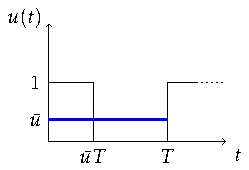
\includegraphics[scale=1]{fig_53_duty}
    \end{minipage}
    \begin{minipage}[c]{0.45\textwidth}
    Compute the average value
    \[
    \colavg{\bar{u}_i(t)} = \frac{1}{T/T_s}\sum_{k=1}^{T/T_s}u_i(t+kT_s)
    \]
    \end{minipage}
    }
    \uncover<3->{
    \[
    \begin{aligned}
    \bar{\rho}_i(t+T_s) &= \bar{\rho}_i(t) + \frac{T_s}{L_i} \bigg( f^\text{in}_i(t) - \colavg{\bar{u}_i(t)} f^\text{out}_i(t) \bigg)\\
    \onslide<4->{
    &\text{subj. to constraints from the S-CTM}\\
    & \forall\, i\in\roads\setminus\roadsin,\, \forall\,t\in\mathbb{N}_+\quad \sum_{j\in\neighUp_i}\colavg{\bar{u}_j(t)}\leq 1.}
    \end{aligned}
    \]
    }
    \uncover<4->{
    \emph{Note:} $\roads\setminus\roadsin$ denote the set of \emph{internal roads} in the network.
    }
\end{frame}